\documentclass{article}
\usepackage[utf8]{inputenc}
\usepackage{kotex}
\usepackage{verbatim}
\usepackage{graphicx}

\title{자료구조 HW2}
\author{C211123 이준선}
\date{\today}

\begin{document}
\maketitle

\section{template이란?}
데이터 타입 검사가 매우 엄격하였던 C언어는, 데이터 타입으로 인한 치명적인 오류는 컴파일 단계에서 발견되기 쉽지만, 너무 엄격한 데이터 타입 검사로 인해 추상적인 데이터 타입의 표현 및 코드의 재사용성이 떨어진다는 단점을 가집니다.
template은 C++에서 다양한 데이터 타입의 추상화를 제공하는 아주 강력한 기능입니다. 이러한 데이터 타입의 추상화는 객체지향 프로그래밍(Object Oriented Programming, OOP)에서 매우 중요한 개념 중 하나입니다. 데이터 타입의 추상화는 코드의 재사용성과 간결성을 높이며, 이는 객체 지향 프로그래밍에서 지양하는 중복의 해악을 피하는 것을 도와줍니다.

일반적으로 C++에는 같은 이름의 함수지만 다른 데이터 타입에 대한 연산을 가능케 하도록 오버로딩이란 기능을 지원합니다. 이는 예를 들어 다음 코드와 같습니다.

\begin{verbatim}
int add(int x, int y) {
    	return x + y;
}

double add(double x, double y) {
	    return x + y;
}
\end{verbatim}

add라는 이름의 함수는 int형 인자 두 개를 받고 int형 반환값을 리턴하는 함수 하나와, double형 인자 두 개를 받고 double형 반환값을 리턴하는 함수 하나, 총 두 개가 있습니다. 이는 직관적이지만 동일한 역할을 수행하는 코드가 두 개 이상 존재함으로써, 중복 코드가 되고 재사용성이 떨어지는 코드라 판단할 수 있습니다. 따라서 이를 해결하기 위해 C++에서는 template을 지원하고, 그러므로 다음과 같이 쓰는 것이 좋습니다.
\begin{verbatim}
template <typename T>
T add(T x, T y) {
	    return x + y;
}
\end{verbatim}
위 코드는 template을 통해 데이터 타입 T에 대한 추상적 연산을 가능하게 합니다. template은 위와 같이 강력한 코드의 재사용성을 보장합니다.

한편 C++에서는 두 가지 template 형식이 있습니다. 하나는 함수 template이며, 다른 하나는 클래스 template입니다. 함수 template은 말 그대로 함수에서 사용하는 template이며, 클래스 template은 클래스에서 사용되는 template입니다.
\begin{enumerate}
    \item 함수 template
    
    함수 template은 위에서 소개한 예시처럼 함수의 추상화와 재사용성을 위해 사용됩니다. 한편 함수 template은 다음과 같이 특수한 데이터 타입에 대해서 특수한 행동을 정의할 수도 있습니다.
    \begin{verbatim}
template <typename T>
T add(T x, T y) {
	    return x + y;   
}

template<>
string add(string str1, string str2) {
    	string result = "결과값 :" + str1 + str2;
    	return result;
}
    \end{verbatim}
    위 코드는 template function으로 정의된 add 함수에 대해, 두 string 객체를 parameter로 받는 특수한 경우에 대한 정의를 따로 한 경우입니다. 이 경우 string을 parameter로 넘기면 return x + y란 코드대신 밑에 코드가 작동하겠죠?
    
    \item class template
    
    class template은 class의 일반화이며, class를 대상으로 한 template입니다. class template은 function template과 다르게 명시적으로 template parameter을 작성해줘야 작동이 된다고 합니다. 이유는 각각의 자료형에 대한 함수를 컴파일러가 다 생성해주는 function template과는 달리, class template은 객체를 생성할 때 명시적으로 자료형을 사용자가 표시해야 하는데, 이때 constructor가 class를 construction 위해 class template에 대한 명시적 template parameter가 필요하다고 합니다.
    
    한편 class template에 대한 예제 코드는 다음과 같습니다.
    \begin{verbatim}
template <typename T>
class CPoint {
private:
    	T x; T y;
public:
    	CPoint(T x, T y);
    	void Move(T x, T y);
    	void Print();
};
    \end{verbatim}
    위 코드는 CPoint Class에 대해 각기 다른 자료형에 대한 class를 정의한 코드입니다. 이때 class 객체를 생성할 떄는 다음과 같이 자료형을 명시하면 됩니다.
    \begin{verbatim}
CPoint<int> P1(1, 2);
CPoint<double> P2(1.1, 2.2);
    \end{verbatim}
\end{enumerate}

\section{코드 설명}
\subsection{hw2a}
\begin{verbatim}
#include <iostream>
using namespace std;

template <typename T>
T add(T x, T y) {
    	return x + y;
}

int main() {
    	int intX = 1, intY = 2;
    	double dbX = 3.3, dbY = 4.4;
    	float fX = 09.24, fY = 10.07;
    	cout << add(intX, intY) << endl;
    	cout << add(dbX, dbY) << endl;
    	cout << add(fX, fY) << endl;
    	return 0;
}
\end{verbatim}
hw2a는 main 함수가 동작하도록 function template을 이용해 add function을 구성하는 문제로, T라는 추상적 자료형을 이용해 T 자료형의 두 인자 x, y를 parameter로 받고, 이에 대해 x + y 연산 결과를 리턴하는 함수를 구성했습니다.\\
따라서 main함수에서는 int형 변수인 intX, intY에 대해, double형과 float형 변수인 각각 dbX, dbY와 fx, fy에 대해 동작하는 add 함수가 따로따로 만들어져서 사용할 수 있게 됩니다. 컴파일 단계에서는, 각각의 자료형에 대한 add 함수가 생성됩니다.
\begin{figure} [h]
    \centering
    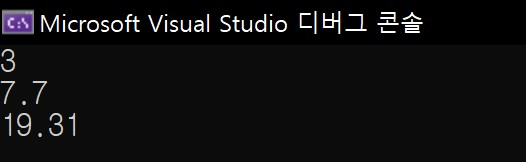
\includegraphics{hw2a result.jpg}
    \caption{hw2a 실행 결과}
    \label{fig:hw2a result}
\end{figure}
Figure \ref{fig:hw2a result}를 보시면, main 함수가 정상적으로 작동한 것을 확인할 수 있습니다. 

\subsection{hw2b}
\begin{verbatim}
#include <iostream>
using namespace std;

template <typename T>
class CPoint {
private:
    	T x; T y;
public:
    	CPoint(T x, T y);
    	void Move(T x, T y);
    	void Print();
};

template<typename T>
CPoint<T>::CPoint(T x, T y)
{
    	this->x = x;
    	this->y = y;
}

template <typename T>
void CPoint<T>::Move(T x, T y) {
    	this->x = x;
    	this->y = y;
}

template<typename T>
void CPoint<T>::Print()
{
    	cout << "(" << this->x << ", " << this->y << ")" << endl;
}


int main() {
        CPoint<int> P1(1, 2);
        CPoint<double> P2(1.1, 2.2);
        P1.Move(2, 3);
        P2.Move(2.2, 3.3);
        P1.Print();
        P2.Print();
        return 0;
}
\end{verbatim}
hw2b는 class template을 이용해 CPoint라는 class를 정의하는 문제였다. function template과 마찬가지로, class 선언부에 T라는 template을 이용하여 class의 추상화를 진행한다. \\
main함수에서는 CPoint\<type\>의 형태로, int와 double 형에 대해 각각 P1, P2라는 CPoint 객체를 생성합니다. P1, P2에 대해, 함수 Move와 Print가 정상적으로 동작함을 알 수 있습니다.
\begin{figure} [h]
    \centering
    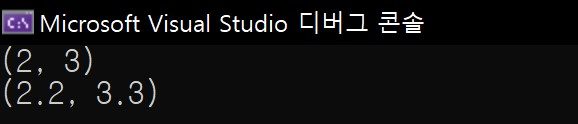
\includegraphics{hw2b result.jpg}
    \caption{hw2b 실행 결과}
    \label{fig:hw2b result}
\end{figure}
figure \ref{fig:hw2b result}를 통해 위 main 함수가 정상적으로 실행되었음을 확인할 수 있습니다.

\subsection{hw2c}
\begin{verbatim}
#include <iostream>
using namespace std;

template <typename T>
class CPoint {
    	T x; T y;
public:
    	T getXpos();
    	T getYpos();
    	CPoint(T x, T y);
    	void Move(T x, T y);
    	template<typename U>
    	friend std::ostream& operator << (std::ostream& rst, CPoint& p);
};

template<typename T>
T CPoint<T>::getXpos()
{
    	return this->x;
}

template<typename T>
T CPoint<T>::getYpos()
{
	    return this->y; 
}

template<typename T>
CPoint<T>::CPoint(T x, T y)
{
    	this->x = x;
    	this->y = y;
}

template <typename T>
void CPoint<T>::Move(T x, T y) {
    	this->x = x;
    	this->y = y;
}

template<typename T>
std::ostream& operator<<(std::ostream& rst, CPoint<T>& point)
{
    	rst << "(" << point.getXpos() << ", " << point.getYpos() << ")" << endl;
    
    	return rst;
}


int main() {
    	CPoint<int> P1(1, 11);
    	CPoint<double> P2(1.1, 2.2);
    	P1.Move(8, 13);
    	P2.Move(8.97, 20.39);
    	cout << P1 << P2;
    	return 0;
}

\end{verbatim}
hw2c는 hw2b의 class에서, Print() function 대신 연산자 오버로딩을 통해 $<<$ 연산자를 재정의하는 문제였습니다. 이는 C++의 연산자 오버로딩을 다룰 때 조심할 몇 가지 주의사항만 지킨다면, 연산자 오버로딩을 통해 간단히 해결할 수 있는 문제입니다.

\begin{verbatim}
template <typename T>
class CPoint {
    	T x; T y;
public:
    	T getXpos();
    	T getYpos();
    	CPoint(T x, T y);
    	void Move(T x, T y);
    	template<typename U>
    	friend std::ostream& operator << (std::ostream& rst, CPoint& p);
};
\end{verbatim}
위 class 선언과 정의부에서, operator $<<$ 에 대한 overloading을 하고 있습니다. 참고로 operator$<<$ 가 CPoint 내부에 선언되어 있어 이를 멤버 함수로 착각하기 쉬운데, friend 키워드를 지울 경우 컴파일 단계에서 에러가 발생합니다. operator$<<$ 은 전역 함수이며, 단지 CPoint의 friend로 지정하여 CPoint에 대한 함수 본체를 구현한 것에 불과합니다. \\
한편 operator$<<$ 역시 CPoint에 대한 template이 필요하므로, operator << 위에 template<typename U>를 통해 operator$<<$은 U를 template으로 받는다는 것을 명시했습니다. 이렇게 한 이유는 바로 다음 operator $<<$ 의 정의부를 확인하면 알 수 있습니다.
\begin{verbatim}
template<typename T>
std::ostream& operator<<(std::ostream& rst, CPoint<T>& point)
{
    	rst << "(" << point.getXpos() << ", " << point.getYpos() << ")" << endl;
    
    	return rst;
}
\end{verbatim}
operator$<<$ 의 정의부를 보면, template\<typename T\>를 통해 CPoint\<T\>에 대한 참조 point를 parameter로 넘겨 받음을 알 수 있습니다. template\<typename T\>는 class의 template\<typename T\>와 다른, operator$<<$만의 template이므로, operator<< 선언부에도 동일하게 template\<typename U\>를 써주는 겁니다. 그니깐 U는 operator$<<$ 의 template T를 명시한 것입니다.\\
한편 out stream(출력 스트림)에 대한 참조 rst(result의 약자입니다)를 parameter로 받습니다. rst에다가 출력하고자 하는 out stream을 모두 이어 받고, 최종 결과(출력 스트림)를 return 합니다. 이 방식은 operator$<<$를 overloading할 때 일반적으로 사용되는 방식입니다.

참고로 한편 $>>$ 을 overloading하고 싶다면, 입력 스트림에 대한 참조인 istream& 에 대해 $>>$ 연산으로 입력하고자 하는 스트림을 집어넣은 뒤 return 합니다.

\begin{figure} [h]
    \centering
    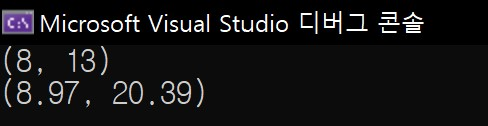
\includegraphics{hw2c result.jpg}
    \caption{hw2c 실행 결과}
    \label{fig:hw2c result}
\end{figure}
Figure \ref{fig:hw2c result}을 보면, 정상적으로 $<<$ 연산에 대해 연산자 overloading이 제대로 작동된 것을 확인할 수 있다.

\end{document}
